\section{Evaluation Metrics} \label{eval}

The F1 score is a metric used to evaluate the performance of many machine learning jobs. It is computed as the harmonic mean of precision and recall, where precision is the ratio of true-positive (TP) predictions to the total positive predictions, and recall is the percentage of true-positive predictions to the total actual positive values. The F1 score is between 0 and 1, with more elevated values representing better performance.
Precision indicates the accuracy of the classifier's prediction of the positive class. It is computed by taking the number of correct positive predictions (True Positive) and dividing it by the total number of positive predictions (True Positive and False Positive). A higher precision value means that the classifier is less likely to identify a negative instance as a positive incorrectly.
Recall measures the classifier's ability to identify all positive instances. It is determined by dividing the number of True Positive predictions by the total number of positive predictions (True Positive and False Negative). A higher recall value indicates that the classifier is less likely to miss a positive instance.

\begin{equation}
    Precision = \frac{TP}{TP + FP}
\end{equation}

\begin{equation}
    Recall = \frac{TP}{TP + FN}
\end{equation}

\begin{equation}
    F1 = \frac{2 * (Precision * Recall)}{Precision + Recall}
\end{equation}

Text-to-SQL tasks are usually evaluated by multiple methods such as Component Matching, Accurate matching rate and Execution accuracy rate. Predicted SQL statements are compared with standard statements to determine how accurate the match is.
By splitting the predicted SQL statement and definitive statement into multiple clauses according to keywords, we can solve the problem of matching errors caused by the order of the where clause. The matching is successful as long as the elements in both sets are the same.

\begin{equation}
    Accuracy = \frac{Successful\ matching\ of\ predicted\ SQL\ statements}{total number\ of\ questions}
    \label{fig:acc1}
\end{equation}

When using the correct predicted SQL statements, the correct execution rate refers to the proportion of questions that can receive the correct answers from the database.

% pics/acc2.png
% \begin{figure}[htb]
%     \centering
%     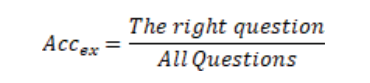
\includegraphics[width=0.4\textwidth]{pics/acc2.png}
%     % \caption{Accuracy rate of the predicted SQL statements}
%     \label{fig:acc2}
% \end{figure}

% By predicting the key F1 values for SQL statements, the model can also be evaluated.

% % pics/f1.png
% \begin{figure}[htb]
%     \centering
%     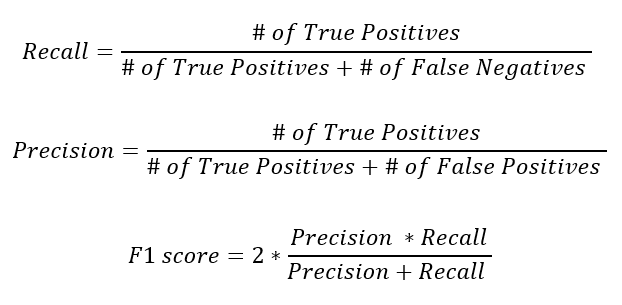
\includegraphics[width=0.6\textwidth]{pics/f1.png}
%     % \caption{F1 score for SQL statements}
%     \label{fig:f1}
% \end{figure}

\subsection*{Evaluation Setup}

The evaluation methods for Text-to-SQL systems have advanced over time to assess different aspects of model performance and adaptability. Early datasets generally used a standard train/dev/test split to randomly divide question-SQL pairs across sets as proposed by Iyer et al. (2017), which provided a baseline for evaluation but did not specifically target model generalization capabilities.

To assess the ability of models to generalize to new SQL query structures within a given domain, Finegan-Dollak et al. (2018) introduced the SQL query split method. This method ensures that SQL queries are only present in one set among the train, dev, and test sets, offering a better understanding of how well models can adapt to new query structures. This approach allows researchers to more accurately evaluate the robustness of their models when faced with novel SQL queries.

In addition to the SQL query split, Yu et al. (2018c) proposed a database split method, which aims to evaluate the generalization capabilities of Text-to-SQL models across different databases. By withholding databases in the test set from the training phase, this method assesses the ability of models to handle unseen databases, emphasizing the importance of real-world adaptability in Text-to-SQL systems.

Other splitting methods have also been proposed to support various research objectives. For example, Shaw et al. (2021) and Chang et al. (2020) have introduced alternative evaluation setups to address specific challenges and research questions in the Text-to-SQL domain. These methods, along with the standard train/dev/test split, SQL query split, and database split, contribute to the diverse range of evaluation strategies employed in Text-to-SQL research, enabling a more comprehensive understanding of model performance and generalization capabilities.


% Question split: split the question-SQL pairs randomly (Iyer et al., 2017).
% SQL query split: no SQL query is allowed to appear in more than one set among the train, dev, and test sets (Finegan-Dollak et al., 2018)
% Database split: databases in the test set do not appear in the training time (Yu et al., 2018c)
% Others (Shaw et al., 2021) (Chang et al., 2020)

\subsection{Naiive Execution Accuracy}

Naïve Execution Accuracy (NEA) has become a popular evaluation metric for Text-to-SQL systems because it can measure the accuracy of generated SQL queries in a way that considers both syntax and meaning. Unlike other metrics that mainly focus on the syntax of the queries, NEA examines the practical impact of the queries by evaluating their execution results. Therefore, it provides a more complete view of a model's performance, allowing researchers to better understand how well their algorithms perform in real-world situations.

By applying NEA to commonly used datasets like GeoQuery, IMDB, Yelp, and WikiSQL, researchers can gain a more nuanced understanding of their models' strengths and weaknesses. For instance, GeoQuery is a dataset that contains geographical questions and corresponding SQL queries. By using NEA to evaluate this dataset, researchers can determine not only whether their model generates syntactically correct SQL queries but also whether these queries return the correct geographical data when executed.

Similarly, NEA provides valuable insight into the performance of Text-to-SQL models when generating queries related to movie and business information in the context of the IMDB and Yelp datasets, respectively. By measuring the accuracy of the execution results, NEA helps researchers identify potential improvement areas, whether in the natural language understanding component or the SQL generation process.

The WikiSQL dataset is another significant example where NEA has been used as an evaluation metric. WikiSQL is a massive dataset derived from Wikipedia's SQL-like tables and contains over 24,000 questions and corresponding SQL queries. Evaluating the performance of Text-to-SQL models on WikiSQL can be challenging due to the dataset's size and complexity. However, NEA enables researchers to assess the performance of their models more, accounting for both the syntax of the generated queries and the accuracy of the data they return when executed.

In summary, the adoption of Naïve Execution Accuracy as an evaluation metric for Text-to-SQL systems has proven to be valuable in recent studies involving datasets such as GeoQuery, IMDB, Yelp, and WikiSQL. By evaluating the practical impact of generated SQL queries, NEA provides a more comprehensive understanding of a model's performance than traditional metrics that concentrate solely on syntax. Consequently, NEA enables researchers to identify potential improvement areas more effectively, ultimately advancing Text-to-SQL technology.

\subsection{Exact String Matching}

Exact Matching\cite{xu_sqlnet_2017}, a popular metric for assessing the effectiveness of Text-to-SQL models, but it has drawbacks because it can yield erroneous negative results when the semantic parser can produce innovative syntactic structures. The predicted SQL query is compared against the corresponding reference SQL query. The model is considered to have produced the proper SQL query and is given a score of 1.0 if the predicted query is an exact duplicate of the reference query. The model is deemed to have generated an invalid query and obtains a score of 0.0 if the predicted query does not match the reference query. This metric aids in evaluating the overall syntactic and semantic accuracy of the generated query, but it ignores the query's constituent parts. This measure is a reliable evaluation technique because it verifies the entire SQL query. It is, therefore, a more stringent evaluation metric because it only deems a query correct if it exactly matches the reference question, down to the capitalization, spacing, and word order.


\subsection{Exact Set Matching}

Exact Set Matching compares the set of predicted SQL queries with the set of corresponding reference SQL queries, regardless of the elements' order, to assess the performance of a model. If every element from the set of predicted queries is included in the reference query, it returns a score of 1.0; otherwise, it returns a score of 0.0.

Generally, Exact Set Matching is more forgiving than Exact Matching, as the former does not take the order of elements or capitalization into account. On the other hand, Exact Matching is more stringent as it requires a perfect match including the order of words, capitalization and spaces, thus making it a reliable evaluation method.


\subsection{Component Matching}

Component matching\cite{yu_spider_2019} involves comparing the elements of the generated SQL query (e.g., the specified columns and tables) to the elements of the reference SQL query. Evaluation is based on the number of components that match correctly between the produced and reference queries, with a higher amount indicating improved performance. This metric assists in measuring the precision of the model's capability to create the correct SQL query components, but it does not factor in the full syntactic or semantic correctness of the query. Furthermore, it is utilized to assess the performance of various models on the same dataset.

\subsection{Test Suite Accuracy (Execution Accuracy)}

The execution accuracy metric\cite{yu_spider_2019} is a commonly used measure to evaluate the performance of text-to-SQL models. It determines the percentage of correctly generated SQL queries that can be successfully executed on the relevant database. In other words, it evaluates how well a model can convert text written in natural language into a SQL query that can successfully access the desired data from a database.

Execution accuracy is typically reported as a percentage, and higher values denote better performance. It is also important to remember that this metric only considers how correctly the generated SQL queries are syntactically and semantically and ignores how relevant or comprehensive the information is that is returned. Consequently, it is frequently combined with other metrics, such as informativeness, which assesses the accuracy and completeness of the retrieved data.
